\documentclass[11pt, oneside]{article}
\usepackage[letterpaper, margin=2cm]{geometry}
\usepackage{AERE546}
\usepackage{xspace}

\begin{document}
\noindent \textbf{\Large{Caleb Logemann \\
AER E 546 Fluid Mechanics and Heat Transfer I \\
Homework 2
}}

%\lstinputlisting[language=MATLAB]{H01_23.m}
\begin{enumerate}
  \item % #1
    The heat fin equation is the linear o.d.e.
    \[
      \d[2]{T}{x} = MT
    \]
    where $M$ is a sort of thermal mass.
    First write the finite difference equation in terms of a tridiagonal matrix.
    Solve that equation using the Thomas algorithm (Gaussian elimination) for:
    \begin{enumerate}
      \item[(a)] % Done
        Compute a solution with the boundary conditions $T(0) = 1$ and
        $T(1) = 0$.
        This corresponds to a fin that is between a hot and a cold reservoir.
        In non-dimensional terms, the heat flux into the cold reservoir is
        $-\d{T}{x}$ at $x = 1$.
        Obtain the heat flux as $x = 1$ for $M = 1, 5, 9$. Use enough grid
        points to obtain 1\% accuracy.
        Provide your three numerical values of the heat flux.
        Provide a single graph with curves of $T(x)$ for the 3 values of $M$.

        First I will establish a some notation.
        I will discretize the fin into $N + 1$ points.
        Let $x_i = \frac{i}{N}$, then $x_0 = 0$ and $x_N = 1$.
        Let the approximate solution at $x_i$ be represented by $T_i$.
        Then a numerical solution consists of a set of values $T_i$ for
        $i \in \NN$, $0 \le i \le N$.

        Next I will discretize the partial differential equation into a discrete
        equation.
        The second order central finite difference for the second derivative is
        \[
          \frac{T_{i - 1} - 2T_i + T_{i+1}}{\Delta x^2}
        \]
        Plugging this into the partial differential equation gives the following
        difference equation
        \[
          \frac{T_{i - 1} - 2T_i + T_{i+1}}{\Delta x^2} = MT_i
        \]
        Simplifying this gives
        \[
          T_{i - 1} + \p{- 2 - M\Delta x^2}T_i + T_{i+1} = 0
        \]

        For this problem the boundary conditions are $T(0) = 1$ and $T(1) = 0$.
        This can be encoded into the numerical solution at $T_0 = 1$ and
        $T_N = 0$.
        Now only the values for $T_i$ for $1 \le i \le N - 1$ need to be found.
        These can be found by solving the equations
        \[
          T_{i - 1} + \p{- 2 - M\Delta x^2}T_i + T_{i+1} = 0
        \]
        for $i = 1$, this become
        \[
           \p{- 2 - M\Delta x^2}T_1 + T_2 = -1
        \]
        and for $i = N - 1$ the equation is
        \[
          T_{N - 2} + \p{- 2 - M\Delta x^2}T_{N - 1} = 0
        \]
        These equation can be written in matrix form as
        \[
          \begin{bmatrix}
            -2 - \Delta x^2 & 1 & & & 0 \\
            1 & -2 - \Delta x^2 & 1 &  \\
             & \ddots & \ddots & \ddots &  \\
             &  & 1 & -2 - \Delta x^2  & 1  \\
            0 &  &  & 1 & -2 - \Delta x^2
          \end{bmatrix}
          \begin{bmatrix}
            T_1 \\
            T_2 \\
            \vdots \\
            T_{N - 2} \\
            T_{N - 1}
          \end{bmatrix}
          =
          \begin{bmatrix}
            -1 \\
            0 \\
            \vdots \\
            0 \\
            0
          \end{bmatrix}
        \]
        This is a tridiagonal system which can be solved easily with the
        Thomas algorithm.

        The following function evaluates the Thomas algorithm on a tridiagonal system.
        \lstinputlisting[language=MATLAB]{tridiag.m}
        The following script uses the previous function to run the Thomas
        algorithm on the tridiagonal system that was found earlier.
        \lstinputlisting[language=MATLAB, lastline=33]{H02.m}
        This script outputs the following image, which shows the three plots
        for $M = 1, 5, 9$.
        \begin{center}
          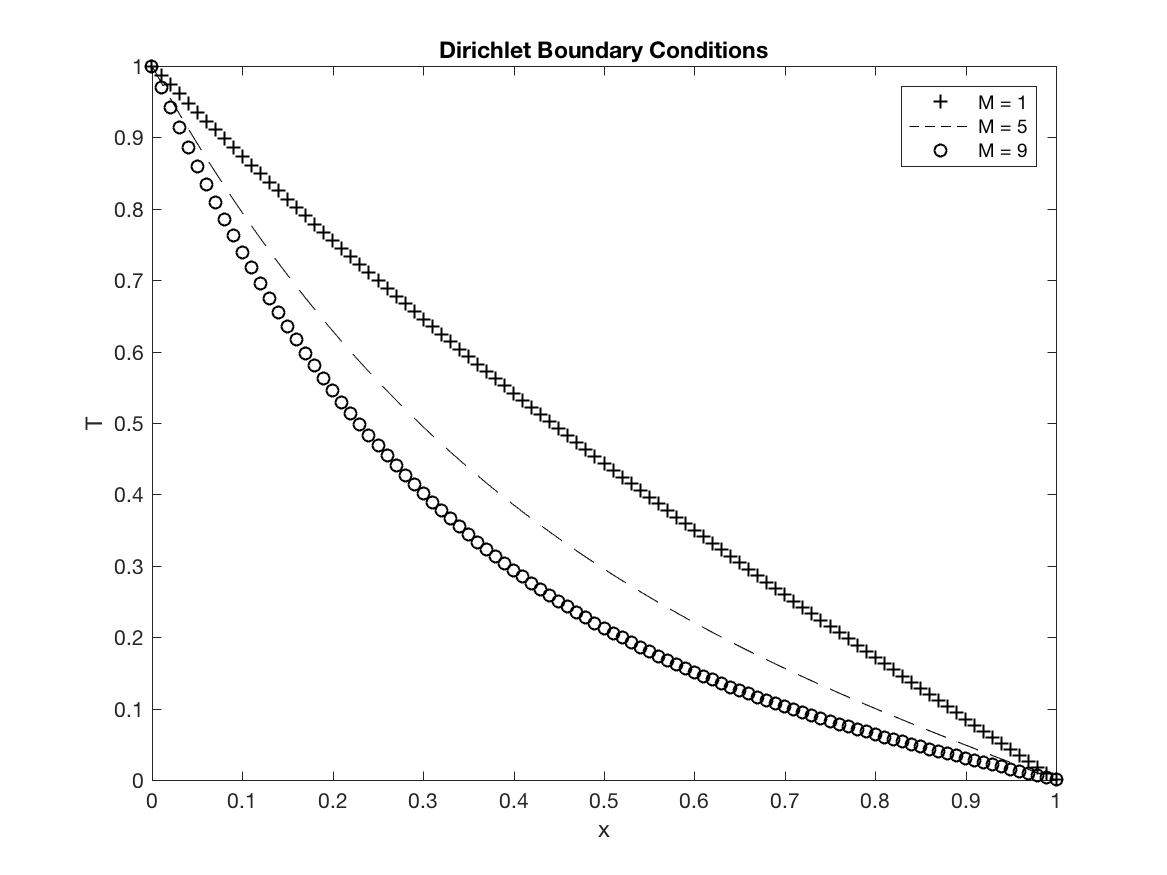
\includegraphics[scale=.5]{Figures/02_01.png}
        \end{center}
        The values of the heat flux at $x = 1$ are given to be
        \begin{align*}
          M &= 1 \qquad \eval{\p{-\d{T}{x}}}{x = 1}{} = 0.850933420029442 \\
          M &= 5 \qquad \eval{\p{-\d{T}{x}}}{x = 1}{} = 0.483548793162072 \\
          M &= 9 \qquad \eval{\p{-\d{T}{x}}}{x = 1}{} = 0.299532256416841
        \end{align*}
        Note that these values are found by evaluating
        \[
          \eval{\p{-\d{T}{x}}}{x = 1}{} \approx \frac{T_{n-1} - T_n}{\Delta x}
        \]

      \item[(b)] % Done
        Compute a solution with the boundary conditions
        $T(0) = 1$, $\d{T(1)}{x} = 0$.
        This corresponds to a fin that is insulated at one end.
        Solve for the temperature, $T(1)$, at the insulated end for
        $M = 1, 5, 9$.
        Provide your three numerical values of $T(1)$.
        Also plot $T(x)$ for $M = 9$ with each pair of boundary conditions and
        compare to the exact solution.

        For this problem we begin with the same difference equation as in part (a).
        \[
          T_{i - 1} + \p{- 2 - M\Delta x^2}T_i + T_{i+1} = 0
        \]
        Again we have the boundary condition that $T(0) = 1$, in results in
        the same modified equation for $i = 1$.
        \[
           \p{- 2 - M\Delta x^2}T_1 + T_2 = -1
        \]
        However we have a different boundary condition at $x = 1$.
        In this case we wish to enforce $\d{T(1)}{x} = 0$.
        In order to enforce this consdition we will consider an
        imaginary point on the fin $T_{N + 1}$, this point doesn't actually
        exist on the fin, but if it did exist and the first derivative was
        zero then
        \[
          \frac{T_{N + 1} - T_N}{\Delta x} = 0.
        \]
        In other words the finite difference for the first derivative
        should be zero, this simplifies to $T_N = T_{N + 1}$.
        This should make intuitive sense, as if the derivative is zero the value
        shouldn't change past then endpoint.
        Using this condition in the difference equation for $i = N$ gives
        \begin{align*}
          T_{N - 1} + \p{- 2 - M\Delta x^2}T_N + T_{N+1} &= 0 \\
          T_{N - 1} + \p{- 2 - M\Delta x^2}T_N + T_{N} &= 0 \\
          T_{N - 1} + \p{-1 - M\Delta x^2}T_N &= 0
        \end{align*}
        We now have $N$ equations for $N$ unknowns.
        This forms the following matrix equation.
        \[
          \begin{bmatrix}
            -2 - \Delta x^2 & 1 & & & 0 \\
            1 & -2 - \Delta x^2 & 1 &  \\
             & \ddots & \ddots & \ddots &  \\
             &  & 1 & -2 - \Delta x^2  & 1  \\
            0 &  &  & 1 & -1 - \Delta x^2
          \end{bmatrix}
          \begin{bmatrix}
            T_1 \\
            T_2 \\
            \vdots \\
            T_{N - 1} \\
            T_{N}
          \end{bmatrix}
          =
          \begin{bmatrix}
            -1 \\
            0 \\
            \vdots \\
            0 \\
            0
          \end{bmatrix}
        \]
        Note that this system is one equation larger than in part (a) as
        the value of $T_N$ must be found.
        Still this is a tridiagonal system that can be solved using the Thomas
        algorithm, which was shown in part (a).
        The following script using the Thomas algorithm to solve this system for
        $M = 1, 5, 9$.
        \lstinputlisting[language=MATLAB, firstline=35, lastline=62]{H02.m}
        The script output the following images.
        Note that the numerical solutions and the exact solutions are
        almost indistinguishable.
        \begin{center}
          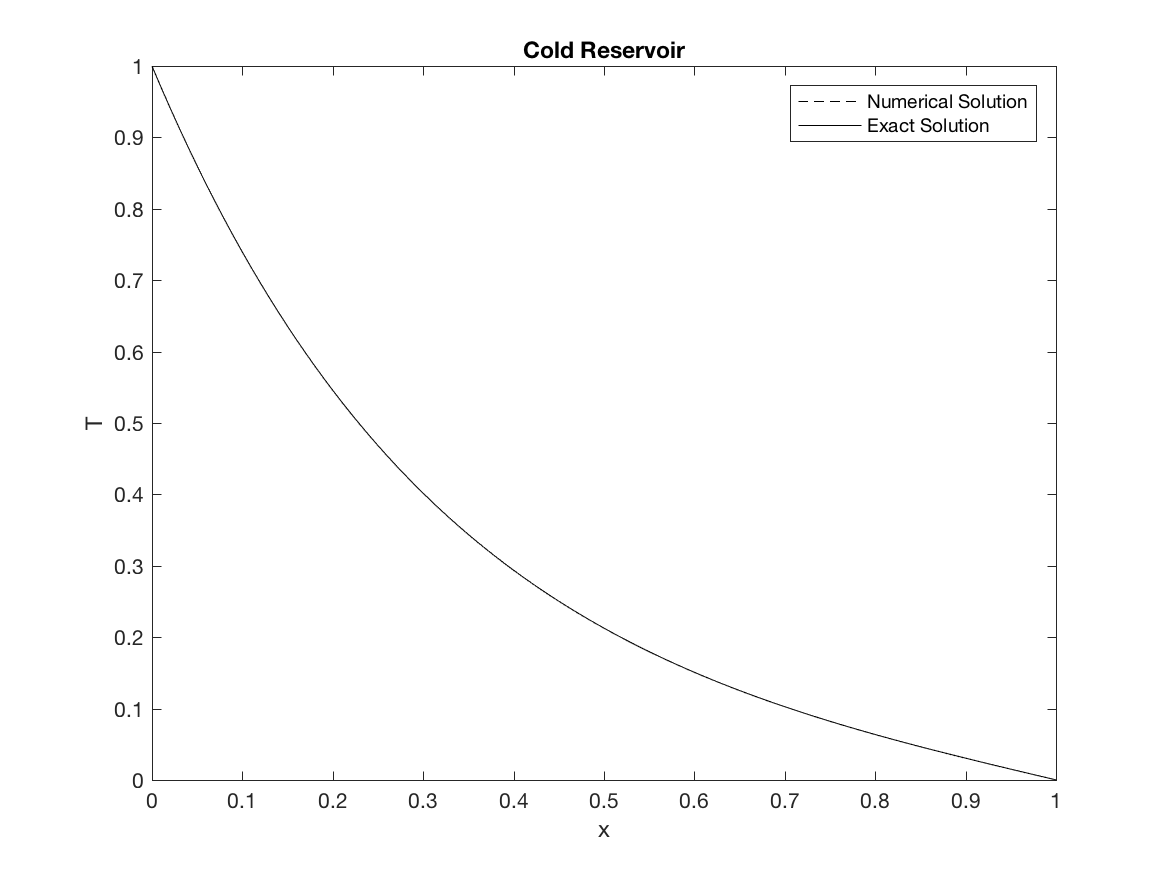
\includegraphics[scale=0.5]{Figures/02_02.png}
          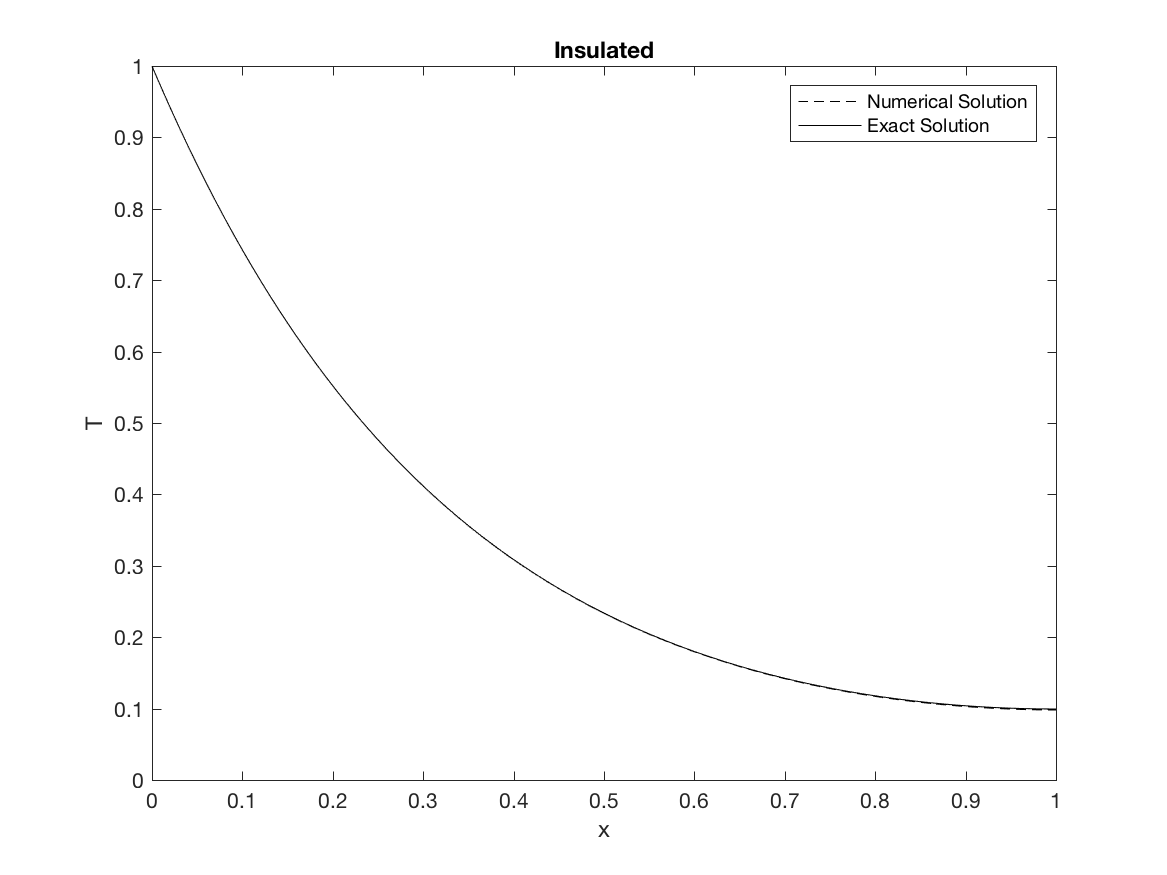
\includegraphics[scale=0.5]{Figures/02_03.png}
        \end{center}
        The following are the numerical values found for $T(1)$ for
        $M = 1, 5, 9$.
        \begin{align*}
          M &= 1 \qquad T(1) = 0.645597948372887 \\
          M &= 5 \qquad T(1) = 0.209066847236553 \\
          M &= 9 \qquad T(1) = 0.097878298010251
        \end{align*}

      \item[(c)]
        Add a distributed heat source: Compute and plot a solution of the
        non-homogeneous equation
        \[
          \d[2]{T}{x} = MT - 100 x^2 \p{1 - x}^2
        \]
        with $M = 9$, $T(0) = 1$ and $\d{T(1)}{x} = 0$.

        In this problem we can start with the tridiagonal system given in (b)
        however the heat source requires changing the RHS.\

        Now the equation for each point $i$ becomes
        \[
          T_{i - 1} + \p{- 2 - M\Delta x^2}T_i + T_{i+1} = -100x_i^2 \p{1 - x_i}^2 \Delta x^2.
        \]
        The equation for $i = 1$ is
        \[
         \p{- 2 - M\Delta x^2}T_1 + T_2 = -100x_1^2 \p{1 - x_1}^2 \Delta x^2 - 1
        \]
        and the equation for $i = N$ is
        \[
          T_{N - 1} + \p{-1 - M\Delta x^2}T_N = -100x_N^2 \p{1 - x_N}^2 \Delta x^2.
        \]
        This create the following tridiagonal system.
        \[
          \begin{bmatrix}
            -2 - \Delta x^2 & 1 & & & 0 \\
            1 & -2 - \Delta x^2 & 1 &  \\
             & \ddots & \ddots & \ddots &  \\
             &  & 1 & -2 - \Delta x^2  & 1  \\
            0 &  &  & 1 & -1 - \Delta x^2
          \end{bmatrix}
          \begin{bmatrix}
            T_1 \\
            T_2 \\
            \vdots \\
            T_{N - 1} \\
            T_{N}
          \end{bmatrix}
          =
          \begin{bmatrix}
            -1 - 100x_1^2 \p{1 - x_1}^2 \Delta x^2 \\
            -100x_2^2 \p{1 - x_2}^2 \Delta x^2\\
            \vdots \\
            -100x_{N-1}^2 \p{1 - x_{N-1}}^2 \Delta x^2\\
            -100x_N^2 \p{1 - x_N}^2 \Delta x^2
          \end{bmatrix}
        \]
        The following script solves the previous tridiagonal system using the
        Thomas algorithm.
        \lstinputlisting[language=MATLAB, firstline=73]{H02.m}

    \end{enumerate}

  \item % #2
    \begin{enumerate}
      \item[(i)]
        What type of p.d.e.\ is
        \[
          \mpd[2]{\phi}{\partial x \partial y} + \phi = 25?
        \]

      \item[(ii)]
        What type of p.d.e.\ does the velocity potential, $\phi$, satisfy if
        \[
          \pd{u}{x} + \pd{v}{y} = 0
        \]
        with
        \[
          u = \pd{\phi}{x} \qquad v = \pd{\phi}{y}?
        \]

      \item[(iii)]
        The boundary layer momentum equation is
        \[
          u \pd{u}{x} + v \pd{u}{y} = \frac{1}{Re} \pd[2]{u}{y}
        \]
        where $Re$ is the Reynolds number.
        What type is this equation?
    \end{enumerate}
\end{enumerate}
\end{document}
